\section{The Font Machinery}
\label{sec:fontmachinery}
We saw in the previous Sections that Oberon texts support attribute specifications (“looks”) for
characters. Three different attributes are supported: font, color, and vertical offset. Let us first
focus on the font attribute. A font can be regarded as a style the standard character set is designed in.
Typically, an entire text is typeset in a single style, that is, there is one font per text. However,
sometimes, an author wants to emphasize titles or words by changing the size of the font or by
varying it to bold face or italics. In special texts, special characters like mathematical symbols or
other kinds of icons may occur. In even more complex documents, mathematical or chemical formulae
might flow within the text.

This generalized view leads us to a different interpretation of the notion of font. We can regard a
font as an indexed library of (graphical) objects, mostly but not necessarily glyphs. In the case of
ordinary characters it is natural to use the ASCII-code as an index, ending up with an interpretation
of text as sequence of pairs (library, index). Note that this is a very general view indeed that, in
principle, is equivalent with defining text as sequence of arbitrary objects.

The imaging model of characters provides 2 levels of abstraction. On the first level, characters are
black boxes specified by a set of metric data \verb|x, y, w, h|, and \verb|dx|. \verb|(x, y)| is a
vector from the current point of reference on the base line to the origin of the box. \verb|w| and
\verb|h| are width and height of the box, and \verb|dx| is the distance to the point of reference of
the next character on the same base line. On the second level of abstraction, a character is defined
by a digital pattern or glyph that is to be rendered into the box. Fig \ref{fig:character} visualizes
this model of characters.

The additional 2 character attributes color and vertical offset appear now as parameters for the
character model. The vertical offset allows translating the glyph vertically and the color attribute
specifies the foreground color of the pattern.
\begin{figure}[h!]
  \label{fig:character}
  \centering
  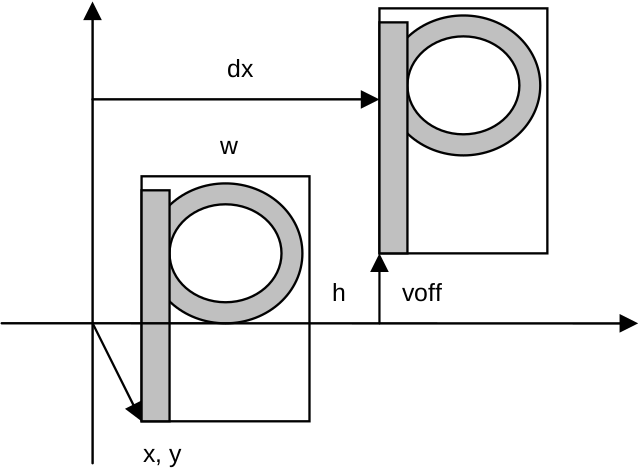
\includegraphics[width=.7\textwidth]{i/i}
  \caption{The geometric character model}
\end{figure}

Good examples of procedures operating on the first level of abstraction are procedures \verb|LocateChar|
and \verb|Width| that we discussed in the previous section, as well as text formatters for a remote
printer.  In contrast, procedure \verb|DisplayLine| operates on the second level.

The representation of characters as digital patterns is merely the last step in a complex font design
and rendering process. At the beginning is a generic description of the shape of each character in
the form of outlines and hints. Outlines are typically composed of straight lines and spline-curves.
Hints are included to assist the digitizer in its effort to faithfully map the filled character outlines
into the device raster. For example, hinting can guarantee consistency of serif shapes and stem widths
across an entire font within a text, independent of the relative positions of the characters with
respect to the grid lines. Automatic digitization produces digital patterns of sufficiently high quality
for printing media resolutions. For screen resolutions, however, we prefer to add a hand-tuning
step. This is the reason why digital patterns are not produced "on the fly" in Oberon.

Oberon's font management is encapsulated in module \verb|Fonts|, with a low-level extension into the
module \verb|Display| that we already know from Chapter \ref{ch:display}. The interface to module
\verb|Fonts| is very simple and narrow:

\begin{verbatim}
  MODULE Fonts;
    TYPE Font = POINTER TO FontDesc;
    FontDesc = RECORD
      name: ARRAY 32 OF CHAR;;
      height, minX, maxX, minY, maxY: INT;
      next: Font
    END;
    VAR Default: Font;
    PROC GetPat(fnt: Font; ch: CHAR; VAR dx, x, y, w, h, patadr: INT);
    PROC This (name: ARRAY OF CHAR): Font;
    PROC Free;
  END Fonts.
\end{verbatim}

Variable name in type \verb|Font| is the name of the underlying file. The variables \verb|height|,
\verb|minX|, \verb|maxX|, \verb|minY|, and \verb|maxY| designate line height and summary metric data.
\verb|Default| is a system-wide default font. It is installed at system loading time. \verb|GetPat|
delivers the geometric data for a given character in a given font (see Fig \ref{fig:extensions}).
This is a procedure to internalize (load) a font from a file given by its name. \verb|Free| releases
from storage fonts that are no longer needed.

Type \verb|Font| should again be regarded as an abstract data type with two intrinsic operations
\verb|This| and \verb|GetPat|. Thinking of the immutable nature of fonts, multiple internal copies
of the same font are certainly undesirable. Therefore, internalized fonts are cached in a private list
that manifests itself in a private field \verb|next| in type \verb|FontDesc|. The cache is maintained
by the internalizing procedure \verb|This| according to the following scheme:
\begin{verbatim}
  search font in cache;
  IF found THEN return cached internalization
  ELSE internalize font; cache it END
\end{verbatim}
The implementation of type \verb|Font| did not raise many challenges. One, however, is an undesirable
side-effect of caching. The problem arises if a font is used for a limited time only. Because it is
referenced by the cache it will never be collected by the system's garbage collector. Two possible
solutions offer themselves: a) provide an explicit freeing operation and b) enforce some special
handling by the garbage collector based on a concept of "weak" pointers.

We conclude this section with a formal specification of the font file format. Note that on the one
hand, the file format is completely private to the managing \verb|Fonts| module and on the other hand,
it should be ultimately stable because it is probably used for long-term backup and for wide-range
data exchange across multi-system platforms.

This is an EBNF specification of the Oberon font file format:
\begin{verbatim}
  FontFile = ident header contents.
  header = abstraction family variant height minX maxX minY maxY.
  contents = nofRuns { beg end } { dx x y w h } { rasterByte }.
\end{verbatim}
\verb|ident|, \verb|abstraction|, \verb|family|, and \verb|variant| are one-byte values indicating
file identification, abstraction (first level without raster bytes, second level with raster bytes),
font family (Times Roman, Oberon, etc.), and variant (bold face, italics etc.). The values
\verb|height|, \verb|minX|, \verb|maxX|, \verb|minY| and \verb|maxY| are 2 bytes long each.
They define in turn line height, minimum x-coordinate (of a box), maximum x-coordinate, minimum
y-coordinate, and maximum y-coordinate. All values in production contents are 2 bytes long.
\verb|nofRuns| specifies the number of runs within the ASCII-code range (intervals occupied without
gaps) and every pair \verb|[beg, end)| describes one run. The tuples \verb|(dx, x, y, w, h)| are
the metric data of the corresponding characters (in their ASCII-code order), and the sequence of
\verb|rasterByte| gives the total of raster information.

In summary, fonts in Oberon are indexed libraries of objects. The objects are descriptions of
character images in 2 levels of abstraction: As metric data of black boxes and as binary patterns
(glyphs). Type \verb|Font| is an abstract data type with intrinsic operations to internalize and
to get character object data. Internalized fonts are cached in a private list.
